
\section{SIMULADOR E TESTES}

O desenvolvimento e os testes utilizaram o simulador no
time da UNESP-Bauru previamente existente. O simulador
executa o módulo de estratégia e o de controle, oriundos do
software executado para o ambiente real, sem alterações nos
códigos. Apenas os arquivos de códigos dos dois módulos
(estratégia e controle) da pasta de fontes destinado ao ambiente
real precisam ser transportados para a pasta do simulador,
nenhuma outra alteração precisa ser realizada. Apesar da
dinâmica ser pouco considerada neste simulador, ele simplifica
a realização de testes dos algoritmos em desenvolvimento, sem
a necessidade da montagem do ambiente real. Uma imagem do
simulador em uma situação de jogo pode ser na vista na Fig. 5.
O simulador pode também apresentar o campo potencial
gerado pelo módulo de controle, Fig. 6.

% FIGURA 5
\begin{figure}[!htb]
\centering
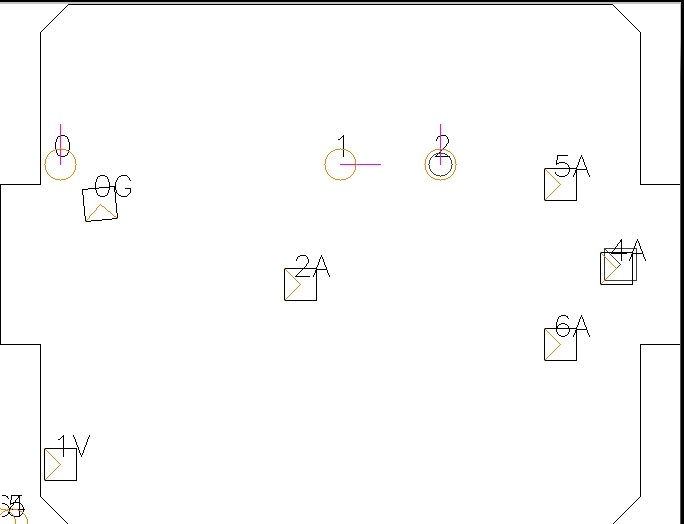
\includegraphics[scale=0.4]{simulador.png}
\caption{Situação representada pelo simulador.}
\label{Rotulo}
\end{figure}
%%%

% FIGURA 6
\begin{figure}[!htb]
\centering
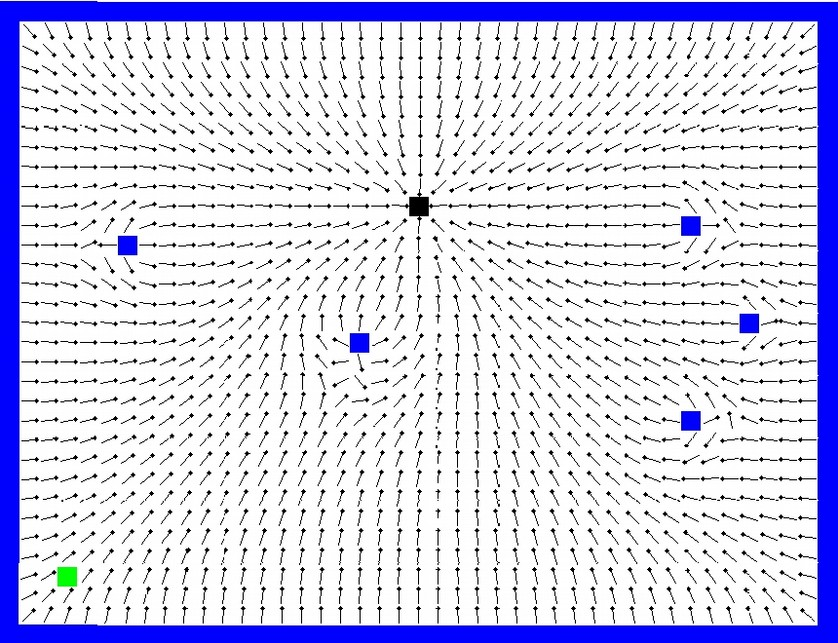
\includegraphics[scale=0.3]{simulador_CP.png}
\caption{Representação do campo potencial para a situação apresentada na
Fig. 5 considerando o robô 1V (volante). Nos quais os quadrados preto, verde
e azul representam respectivamente meta, robô e obstáculo.}
\label{Rotulo}
\end{figure}
%%%

Para que os teste pudessem gerar análises convincentes em
relação ao desenvolvimento da estratégia e do controle, foi
necessário acrescentar uma nova funcionalidade que
permitisse dois times jogarem entre si. Para isso foi
desenvolvido no código do simulador a possibilidade de se
comunicar em rede, de tal forma que houvessem dois times
clientes, cada um com sua estratégia e controle, se
comunicando com o servidor do simulador, que efetiva os
comandos enviados por cada cliente, realizando a
movimentação dos robôs e da bola virtualmente, e fazendo o
papel da visão ao fornecer o estado de cada robô para os times
clientes. Para a comunicação entre os clientes e o servidor
optou-se por um protocolo de comunicação simples, o User
Datagram Protocol (UDP).

Desta forma mudou-se a forma como o simulador funciona.
Na Fig. 7 é apresentado o esquema, de forma simplificada, do
simulador antigo, em que a estratégia recebe o estado do robô,
calcula o objetivo e envia para o controle. O controle vai
calcular a trajetória e o comando que será enviado para cada
roda, que será enviado para o simulador que efetua a
movimentação.

% FIGURA 7
\begin{figure}[!htb]
\centering
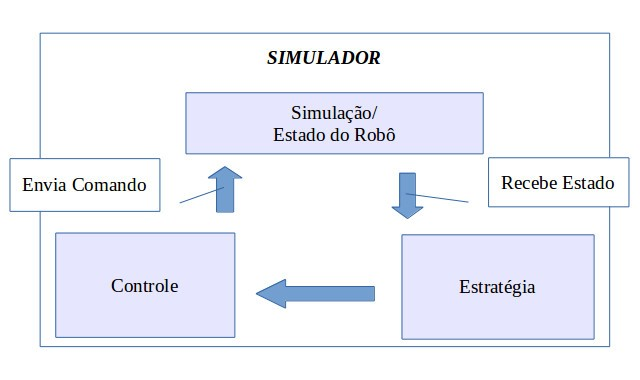
\includegraphics[scale=0.5]{esquema_simulador.png}
\caption{Simulador antes das alterações.}
\label{Rotulo}
\end{figure}
%%%

Na Fig. 8 é apresentado o esquema do simulador atual, no
qual o simulador torna-se um servidor, que recebe os
comandos de cada roda, efetua-os e em seguida envia o estado
do robô para os clientes. Os clientes recebem o estado,
calculam o objetivo através da estratégia e os comandos a ser
enviados para o simulador através do controle, na sequência
esse comando é enviado para o servidor que efetuará a
movimentação dos robôs. Além disso, tem-se a representação
para a conexão de um cliente, mas a representação é a mesma
para dois clientes, que é o caso do futebol de robôs.

% FIGURA 8
\begin{figure}[!htb]
\centering
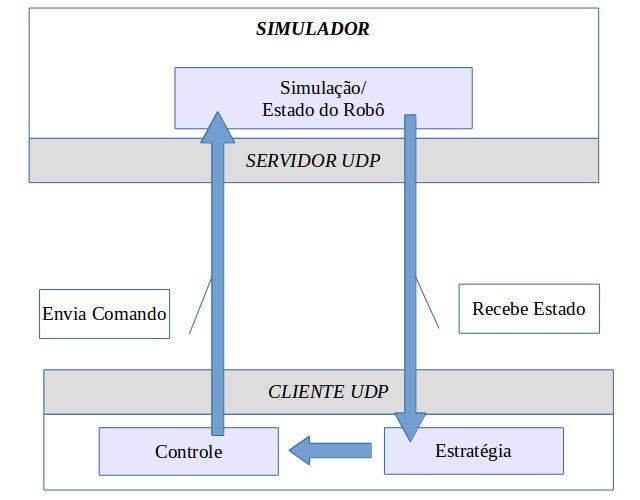
\includegraphics[scale=0.5]{esqumatica_simulador.png}
\caption{ Simulador após alterações, representando uma conexão.}
\label{Rotulo}
\end{figure}
%%%

Assim, o novo simulador permite interação entre dois times
virtuais, levando em consideração a dinâmica, cinemática e
demais constantes físicas referentes ao robô do time Carrossel
Caipira, possibilitando a comparação através de estatísticas
que podem ser coletadas durante a execução do programa, na
figura 9 temos a imagem do novo simulador.

% FIGURA 9
\begin{figure}[!htb]
\centering
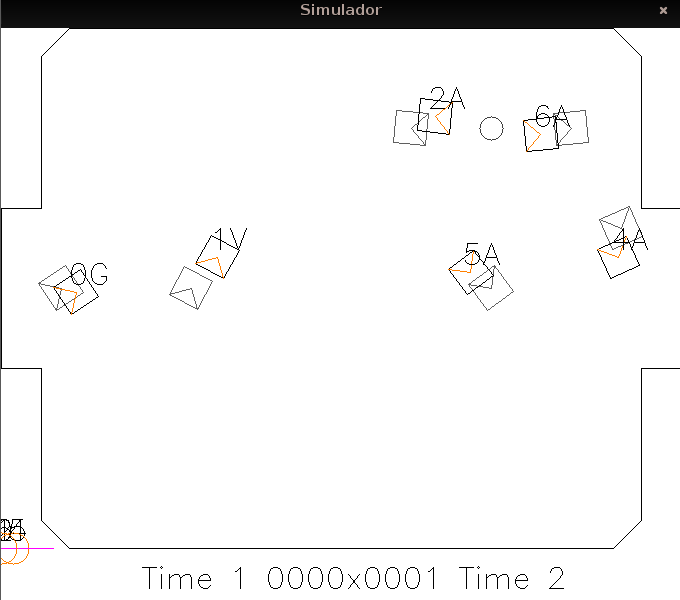
\includegraphics[scale=0.48]{simulador2.png}
\caption{ Simulador após alterações, representando uma conexão.}
\label{Rotulo}
\end{figure}
%%%

Nesta versão, o simulador procura entender o
comportamento da estratégia e controle estudados, através de
situações de jogo como: placar total, gols contra, pênaltis
usufruído pelo time Carrossel Caipira para o desenvolvimento
das pesquisas envolvendo futebol de cometidos, pênaltis
convertidos, gols de cada robô, número de free balls e tempo de
jogo. Além disto, é possível verificar a evolução do placar no
decorrer da simulação e avaliar o intervalo de confiança para
estimar a margem de erro dos dados levantados. A análise
quantitativa dos dados estimula a análise com dados reais feita
no ambiente controlado do laboratório que complementa o
ambiente instrumental robôs. 
